% to compile:
% bibtex proposal
% bibtex proposal
% pdflatex proposal

\documentclass[11pt]{article}
\usepackage{graphicx}
\usepackage{amssymb}
\usepackage{hyperref}
\usepackage{graphicx}
\graphicspath{ {./images/} }

\title{A Domain-Specific Knowledge Graph for News Item Recommendations and Information Retrieval}
\author{Author: Christopher Eaves-Kohlbrenner \\ Supervisor: Michael Zakharyaschev}

\begin{document}
\maketitle

\begin{center}
\hfill \break
\hfill \break
\hfill \break
MSc Data Science project proposal\\
Department of Computer Science and Information Systems\\
Birkbeck College, University of London\\
2021\\
\hfill \break
\hfill \break
\hfill \break

\textit{This report is substantially the result of my own work, expressed in my own words, except where explicitly indicated in the text. I have read and understood the sections on plagiarism in the Programme Handbook and the College web site. I give my permission for it to be submitted to the JISC Plagiarism Detection Service. \\
\hfill \break
The report may be freely copied and distributed provided the source is explicitly acknowledged.}
\end{center}

% \end{center}

\newpage
\begin{abstract}
This proposal introduces the project plan for a knowledge graph in the news domain. The project is intended to build a news knowledge graph to enhance recommendations, link prediction, and information retrieval using semantic technologies, natural language processing, and machine learning.

Two phases are planned: (1) build a prototype of a news knowledge graph using a Reuters archive of 59,542 news items and (2) run experiments aimed at enhancing the knowledge graph to improve recommendation quality and information retrieval. Final outcomes will include a functional graph database application and an evaluation documenting any improvements from the experiments.
\end{abstract}

\newpage
\tableofcontents

\newpage
\section{Introduction}
The goal of this project is to build a knowledge graph for the news domain to improve news item recommendations and information retrieval. Knowledge representation in some form is as old as knowledge itself, but this project will take the world wide web as the modern of knowledge representation. Tim Berners-Lee's invention of the web in 1989 enabled fast electronic access to information, but his vision for a \textit{semantic web} would take that further -- not just raw text on the internet, but machine-readable information to capture semantic meaning.\footnote{ST week 1: \url{https://moodle.bbk.ac.uk/pluginfile.php/1438136/mod_resource/content/2/ST-1.pdf}}

More recently, knowledge graphs have grown rapidly, merging new information into the mathematical graph structure. The last decade has seen notable examples like Wikidata, DBpedia, and the Google Knowledge Graph\cite{farber2015comparative}.

Meanwhile, the media industry generates a high volume of news content that is often unstructured and semantically limited, presenting information retrieval challenges for news consumers and journalists. The data challenges facing news agencies present an opportunity for a domain-specific knowledge graph architecture.

Modeling news items as a knowledge graph requires transforming unstructured text or semi-structured XML into a structured and semantically modelled graph structure, which represents meaning or knowledge in the form of graph nodes and edges. The architecture and storage of knowledge graphs can vary, primarily between RDF stores of subject-predicate-object triples and graph databases like Neo4j\cite{zhao2018architecture}. In either case, this graph structure presents opportunities to enrich the data by creating additional edges or relationships between the various entity nodes.

An effective knowledge graph in the news domain would present benefits similar to Wikidata and others: a machine-readable graph enables others to link data and enrich other data sets; journalists can more easily draw insights about the entities in a story; consumers of the news can retrieve more relevant information and recommendations.

\newpage
\section{Background Research}

\subsection{Literature Review}
\label{sec:LiteratureReview}

A variety of news-specific knowledge systems have been proposed or built to aggregate, generate, and link news data. The efforts described below represent the state of the art for applying knowledge graphs, semantic technology, and natural language processing in the news domain. They form the inspiration for some of the project's architecture and expirementation.

\begin{itemize}
\item \textbf{Neptuno} \cite{castells2004neptuno}, 2004: ``introduction of the emergent semantic-based technologies to improve the processes of creation, maintenance, and exploitation of the digital archive of a newspaper".
\item \textbf{News Engine Web Services (NEWS)} \cite{fernandez2010news}, 2010: a news ontology and metadata vocabulary as tools for handling heterogenous content and customers.
\item \textbf{Global Database of Events, Language, and Tone (GDELT)}\footnote{\url{https://www.gdeltproject.org/}}, 2013: graph of news items and events with real-time monitoring of world's news media.
\item \textbf{Event Registry} \cite{leban2014event}, 2014: ``a system that can analyse news articles and identify in them mentioned world events".
\item \textbf{NewsReader} \cite{vossen2016newsreader}, 2016: a system to read news articles and represent information as RDF; "a cycle of knowledge acquisition and NLP improvement on a massive scale".
\item \textbf{NewsAPI}\footnote{\url{https://newsapi.org/}}, 2017: JSON API to retrieve articles and breaking news headlines from various sources.
\item \textbf{Reuters' Tracer} \cite{liu2017reuters}, 2017 : ``a system that automates end-to-end news production using Twitter data."
\item \textbf{Scalable Understanding of Multilingual MediA (SUMMA)} \cite{germann2018integrating}, 2018: An architecture for monitoring media and applying NLP pipeline.
\item \textbf{Acquisition de Schémas pour la Reconnaissance et l'Annotation d'Événements Liés (ASRAEL)} \cite{rudnik2019searching}, 2019: A system to harvest news text, link to Wikidata, and annotate using IPTC rNews vocabulary.
\item \textbf{News Graph} \cite{liu2019news}, 2019: An enhanced news knowledge graph that adds new entities and relationships and removes news-irrelevant links.
\item \textbf{News Hunter} \cite{berven2020knowledge}, 2020: A knowledge-graph platform and architecture using NLP and ML.
\end{itemize}

The full literature review exercise for the project (\hyperref[sec:PropLiteratureReview]{see Project Plan \#2}) will analyse the news-specific literature above, with a specific focus on research of knowledge graphs, NLP, and statistical ML. This will inform an action plan for the project's knowledge graph architecture and NLP experiments.

In addition to the literature on news-specific knowledge systems, there is a wealth of resources related to knowledge graph architecture more broadly. The literature review will also survey and summarise best practices for knowledge graph architecture:

\begin{itemize}
\item Architecture of knowledge graph construction techniques \cite{zhao2018architecture}
\item A review of relational machine learning for knowledge graphs \cite{nickel2015review}
\item Knowledge graph embedding: A survey of approaches and applications \cite{wang2017knowledge}
\item Knowledge Vault: A Web-Scale Approach to Probabilistic Knowledge Fusion \cite{45634}
\end{itemize}

\subsection{Proof of Concept}
The efforts of this project have already included a preliminary analysis into (1) the available data, (2) initial cleaning of the data, (3) ingestion of a subset of news items into Neo4j, and (4) brief tests of Cypher queries and linked data. \textit{Figure 1} demonstrates this early proof of concept, which will be expanded as documented in the \hyperref[sec:ProposedProject]{``Proposed Project"} and \hyperref[sec:ProjectPlan]{``Project Plan"} below.

This inital proof of concept verifies a few key details:

\begin{itemize}
  \item The chosen technologies--including Neo4j, Cypher, XML documents, and linked Wikidata--can all be applied to this project.
  \item The Reuters archive data set provides a corpus of text documents from which a knowledge graph can be generated, as demonstrated with a subset of 216 news items linked by some simple entities and relationships.
  \item The volume of data will vastly increase the level of effort, from a proof of concept with 216 news items to the full corpus of 59,542 documents.
  \item Many open questions remain around the application of ontologies, linked data, NLP techniques, and evaluation. These open questions will be addressed over the course of the project and outlined in the sections below.
\end{itemize}

\begin{figure}
\centerline{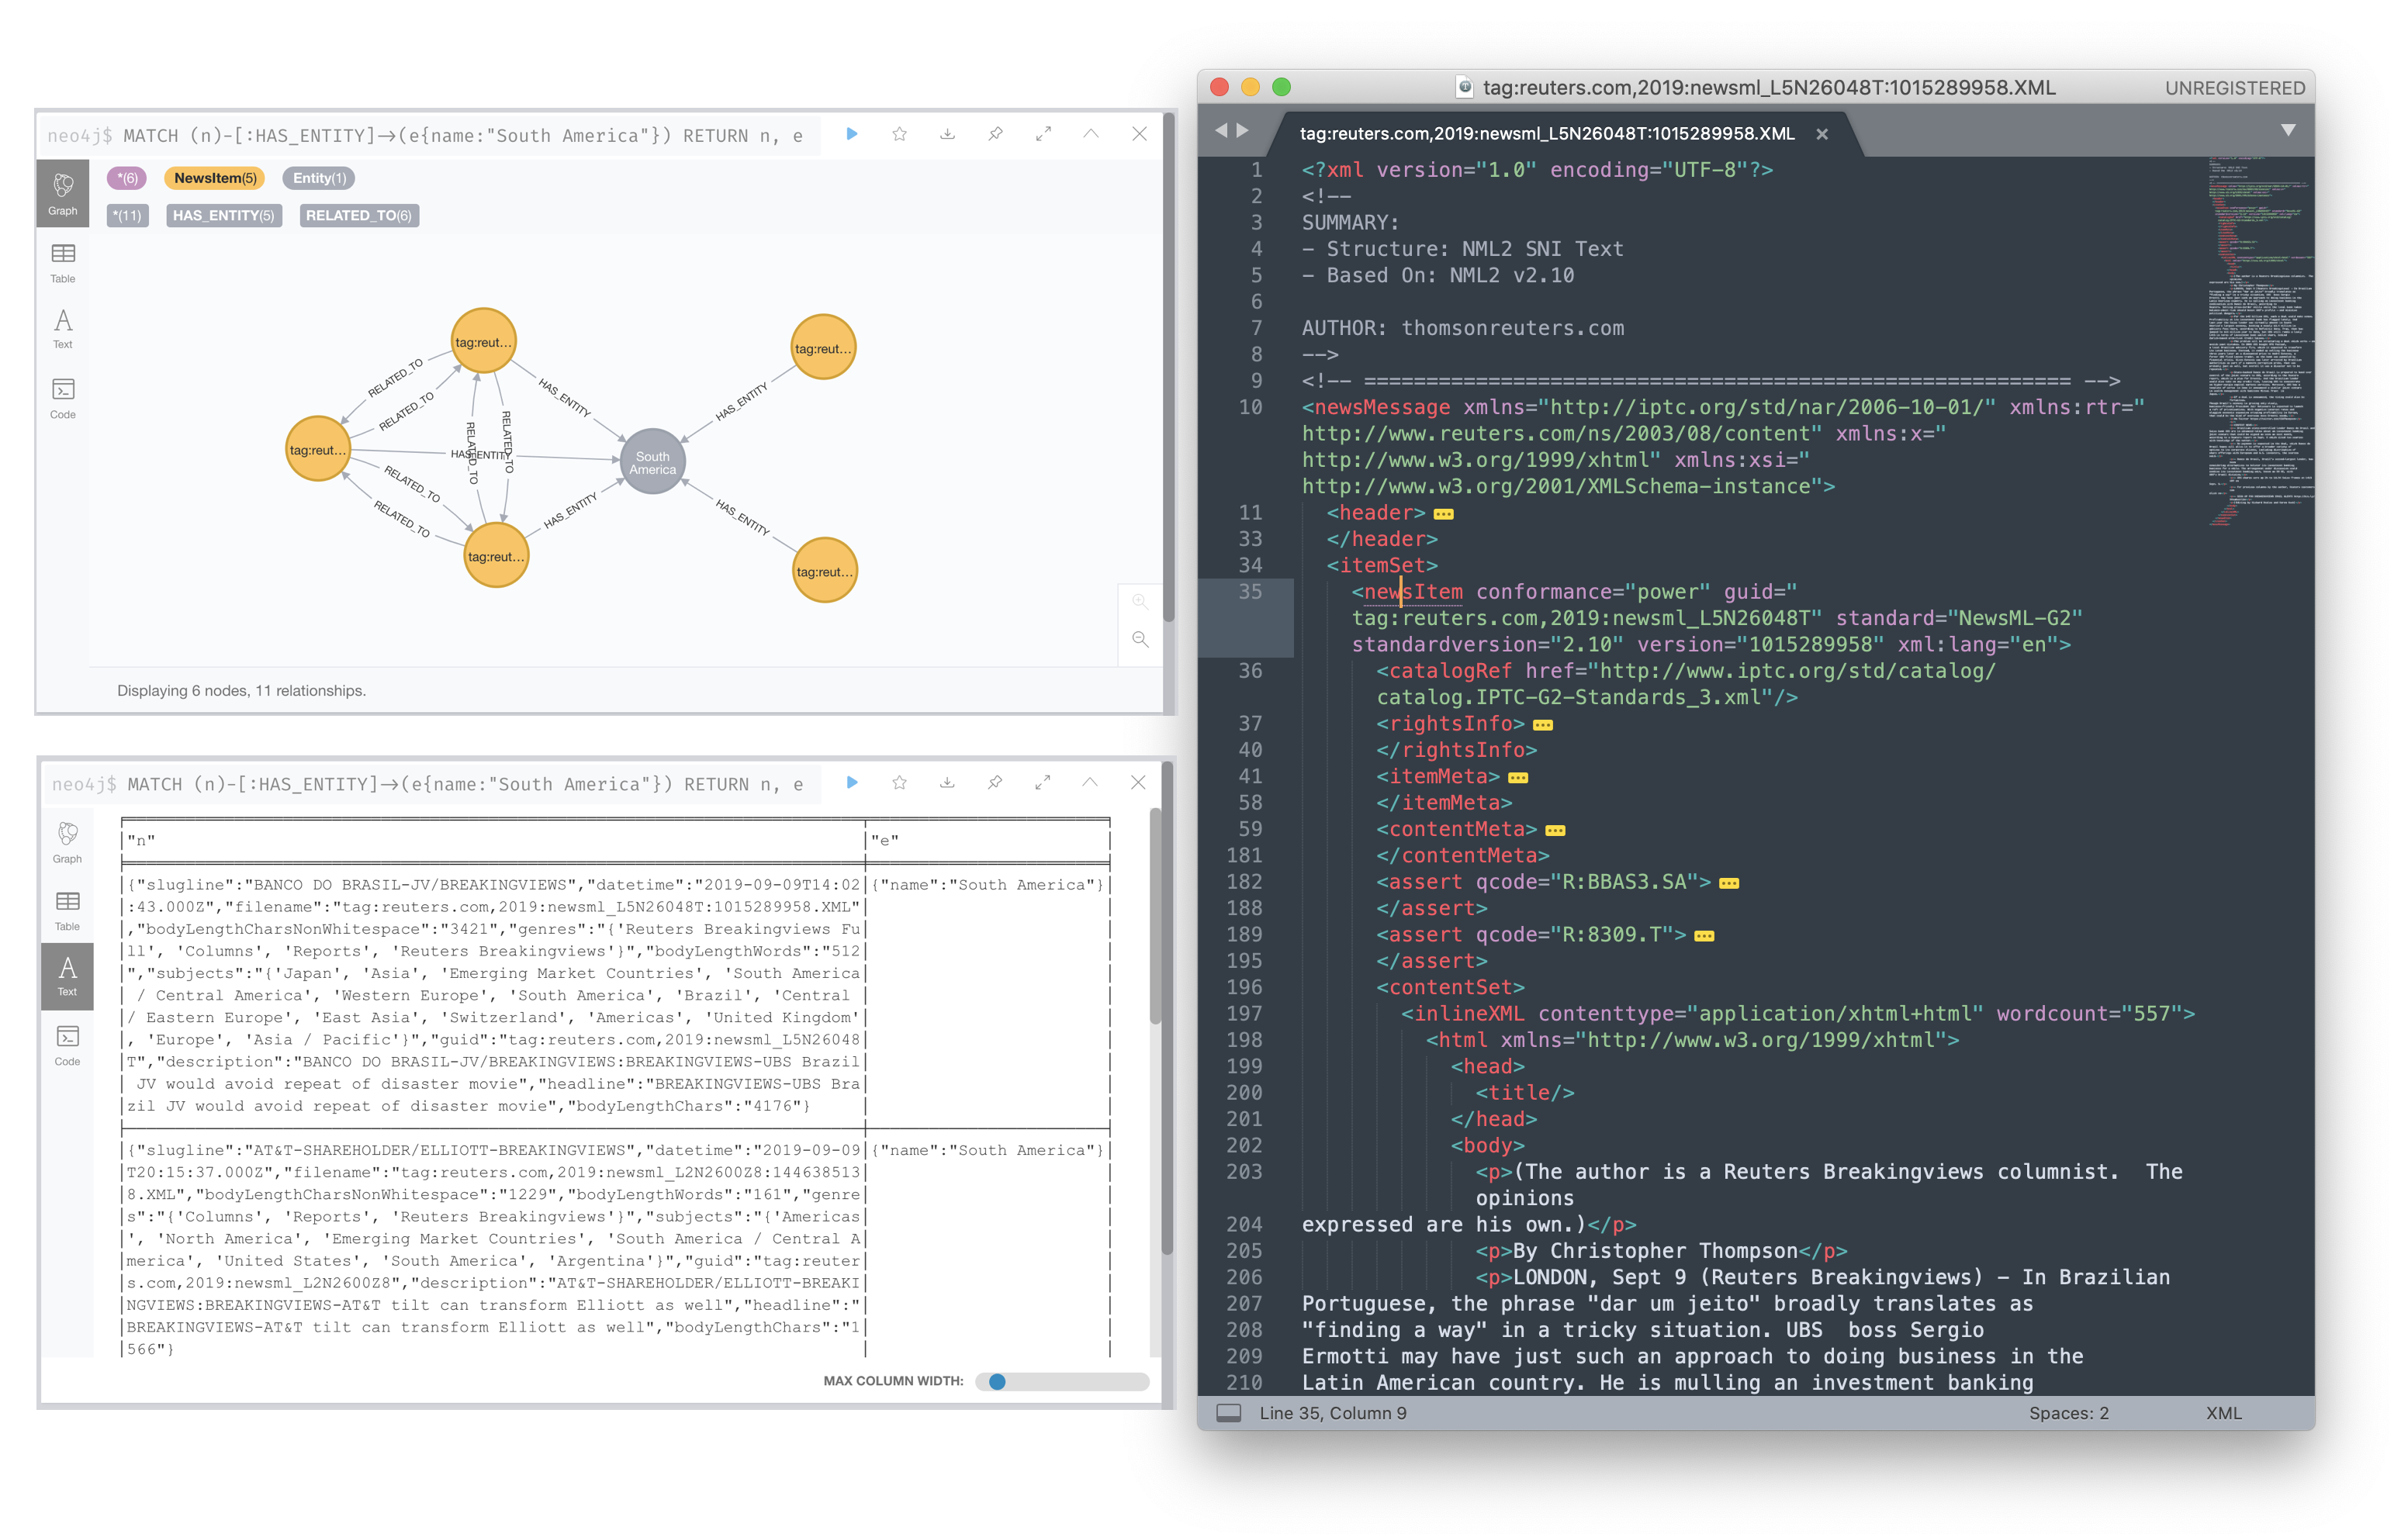
\includegraphics[scale=0.25]{neo4j-proof-of-concept}}
\caption{\textit{The initial knowledge graph proof of concept ingested 216 XML news items into Neo4j and created test relationships between nodes. For example, a news item shown (right) in XML document format matches four other news items via shared entity ``South America", in both graph view (top-left) and table output (bottom-left).}}
\end{figure}

\newpage
\section{Aims and Objectives}
\label{sec:AimsObjectives}

\subsection{Aims}
The \textit{aims} or high-level research questions for this project include:
\begin{itemize}
  \item Design and implement a system for news information retrieval and recommendations
  \item Determine whether and how certain technologies, including knowledge graphs, ontologies, linked data, and natural language processing, can be used to implement such a system
\end{itemize}

\subsection{Objectives}
The \textit{objectives} or concrete and verifiable outcomes include:
\begin{itemize}
  \item Develop a software specification for the design and implementation of an information retrieval system for news XML documents
  \item Build a data extraction pipeline for ingesting news data into the system
  \item Build a knowledge graph prototype stored in Neo4j and query-able via Cypher
  \item Experiment with semantic technologies and natural language processing for entity extraction and link prediction to enhance the knowledge graph
\end{itemize}

\subsection{Additional Details}

This project will build a domain-specific knowledge graph of news items. It will use the knowledge graph to prototype a recommendation system and run experiments to improve recommendations and information retrieval.

The planned experiments include:

\begin{itemize}
\item Apply \textbf{semantic technologies (ST)} including ontologies, vocabulary, and RDF.
\item Apply \textbf{natural language processing (NLP)} techniques including named entity recognition (NER), clustering and similarity, and keyword extraction for topics, key terms, and locations.
\item Apply \textbf{machine learning (ML)} models, including clustering, similarity, and link prediction.
\end{itemize}

The key research question for the initial prototype is: \textbf{Can we build a NewsML to Knowledge Graph pipeline, resulting in a knowledge graph that improves news item recommendations and information retrieval?} This pipeline will transform XML/NewsML documents into a knowledge graph by applying ST, NLP, and ML techniques.

Once the knowledge graph prototype is in place, the ST, NLP, and ML experiments can be run to enhance the knowledge graph. These experiments will investigate some of the following questions:
\begin{itemize}
\item [ST] Can we enhance the data and knowledge graph by authoring or integrating with existing OWL ontologies and RDF linked data?
\item [ST] Can we identify which news item relations are relevant for news? Can we remove irrelevant relations?
\item [ST] Can we determine a meaningful level of connection between news items? For example, one-hop, paths of length N, shared entity with salience above some weight/cutoff.
\item [NLP] Can we enhance the data and knowledge graph with named entity recognition?
\item [NLP/ML] Can we extract latent topics, keywords, and locations from news items, as a \textit{category classification} and/or \textit{latent semantic indexing} task?\footnote{Note to self: see NLP week 10 lecture}
\item [NLP/ML] Can we identify meaningful clusters of news items?
\item [ML] Can we do link prediction to generate new relationships between news items and entities?\footnote{Project will consider 2.2 example of Donald Trump and Lebron James\cite{liu2019news}}
\item [ML] Can we learn Knowledge Graph Embeddings (KGEs), with the intent to "embed components of a KG including entities and relations into continuous vector spaces, so as to simplify the manipulation while preserving the inherent structure of the KG"?\cite{wang2017knowledge}
\item [ML] In addition to the NLP text extraction methods above, can we use probabilistic methods\cite{45634} or Statistical Relational Learning (SRL)\cite{nickel2015review} to build knowledge graph relationships?
\item [evaluation] How can we evaluate improvements in quality or information retrieval? Which metrics are most meaningful among precision, recall, f-score, and similar?\footnote{Project will define its evalution measures. Additional candidate metrics:\\
\url{https://en.wikipedia.org/wiki/Evaluation_measures_(information_retrieval)}}
\item [evaluation] Does the knowledge graph improve information retrieval in terms of precision and recall?
\item [evaluation] Does the knowledge graph improve the quality of recommended news items?
\item [evaluation] Can we expose the knowledge graph as a user-facing application, via Neo4j, a user interface, or API?
\item [evaluation] Does the knowledge graph improve human explainability of news item recommendations?
\end{itemize}

\newpage
\section{Proposed Project}
\label{sec:ProposedProject}
\subsection{Project Technology and Architecture}
Because the project is intended to (1) build a knowledge graph prototype and (2) run NLP experiments to enhance the knowledge graph's news item recommendations and information retrieval, the overall architecture can be viewed as a data pipeline ending in a knowledge graph.

This project will take a "bottom-up" approach, by which data is ingested, other knowledge instances like Wikidata are extracted through linked open data, and the two are fused. This stands in contrast to a "top-down" approach, where an ontology and schema are structured first and knowledge instances are then fit into the structure \cite{zhao2018architecture}. See \textit{Figure 2} for a proposed knowledge graph pipeline and architecture.

\begin{figure}
\centerline{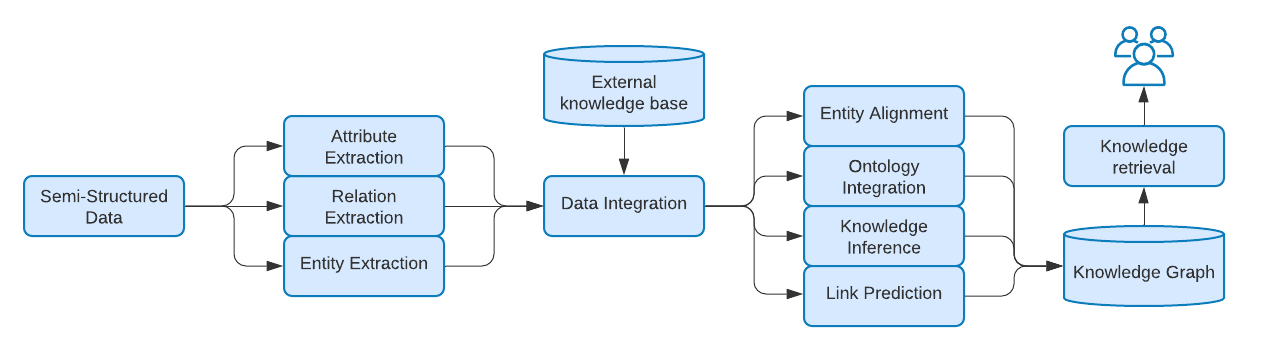
\includegraphics[scale=0.275]{bottom-up-kg-architecture}}
\caption{\textit{High-level architecture of the bottom-up knowledge graph}}
\label{figure:BottomUpKGArchitecture}
\end{figure}

The tech stack will include the following technologies:

\begin{enumerate}
  \item \textbf{Graph database technologies: Neo4j\footnote{\url{https://neo4j.com/}} and the Cypher query language\footnote{\url{https://neo4j.com/developer/cypher/}}}:
  \begin{itemize}
    \item Neo4j is a graph database management system that will enable ingestion of news items to store connected data as nodes and relationships.
    \item The Cypher graph query language can query a Neo4j graph database by matching patterns of nodes and relationships in the graph.
  \end{itemize}
  \item \textbf{Python: Pandas and Neo4j Python driver\footnote{\url{https://neo4j.com/developer/python/}}}:
  \begin{itemize}
    \item The Python programming language enables scripting and data processing, including XML parsing with the built-in \verb+xml.etree.ElementTree+ functions.
    \item The Pandas library will be useful for high-level data analysis in a dataframe to understand the scope and scale of the news item dataset.
    \item The Neo4j Python driver will enable connection to the Neo4j graph database via Python to increase effectiveness over the Neo4j desktop interface.
  \end{itemize}
  \item \textbf{Semantic Technologies: OWL, RDF, Wikidata, Wikifier}:
  \begin{itemize}
    \item OWL
    \item RDF
    \item Wikidata
    \item Wikifier
  \end{itemize}
  \item \textbf{NLP technologies: APOC and scikit-learn}:
  \begin{itemize}
    \item APOC
    \item scikit-learn
  \end{itemize}
\end{enumerate}

Taking a more granular view at the steps from the previous diagram, we can simplify the view to a linear flow of data through the various technologies (\textit{Figure 3}), where the Neo4j interface enables Cypher queries of nodes and relationships (\textit{Figure 4}).

\begin{figure}
\centerline{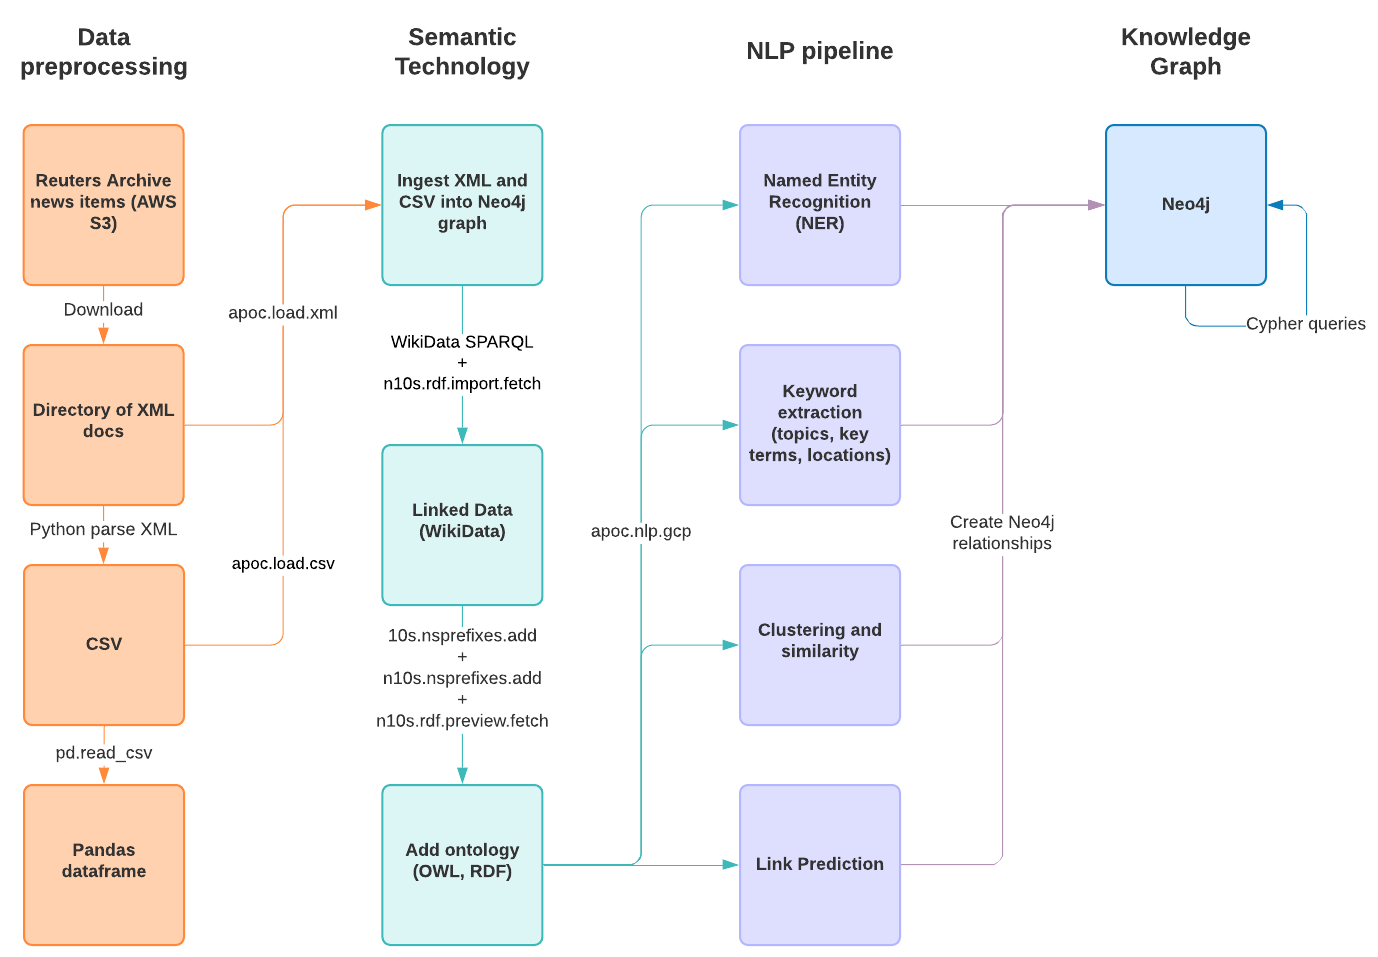
\includegraphics[scale=0.225]{data-pipeline}}
\caption{\textit{Data flow}}
\end{figure}

\begin{figure}
\centerline{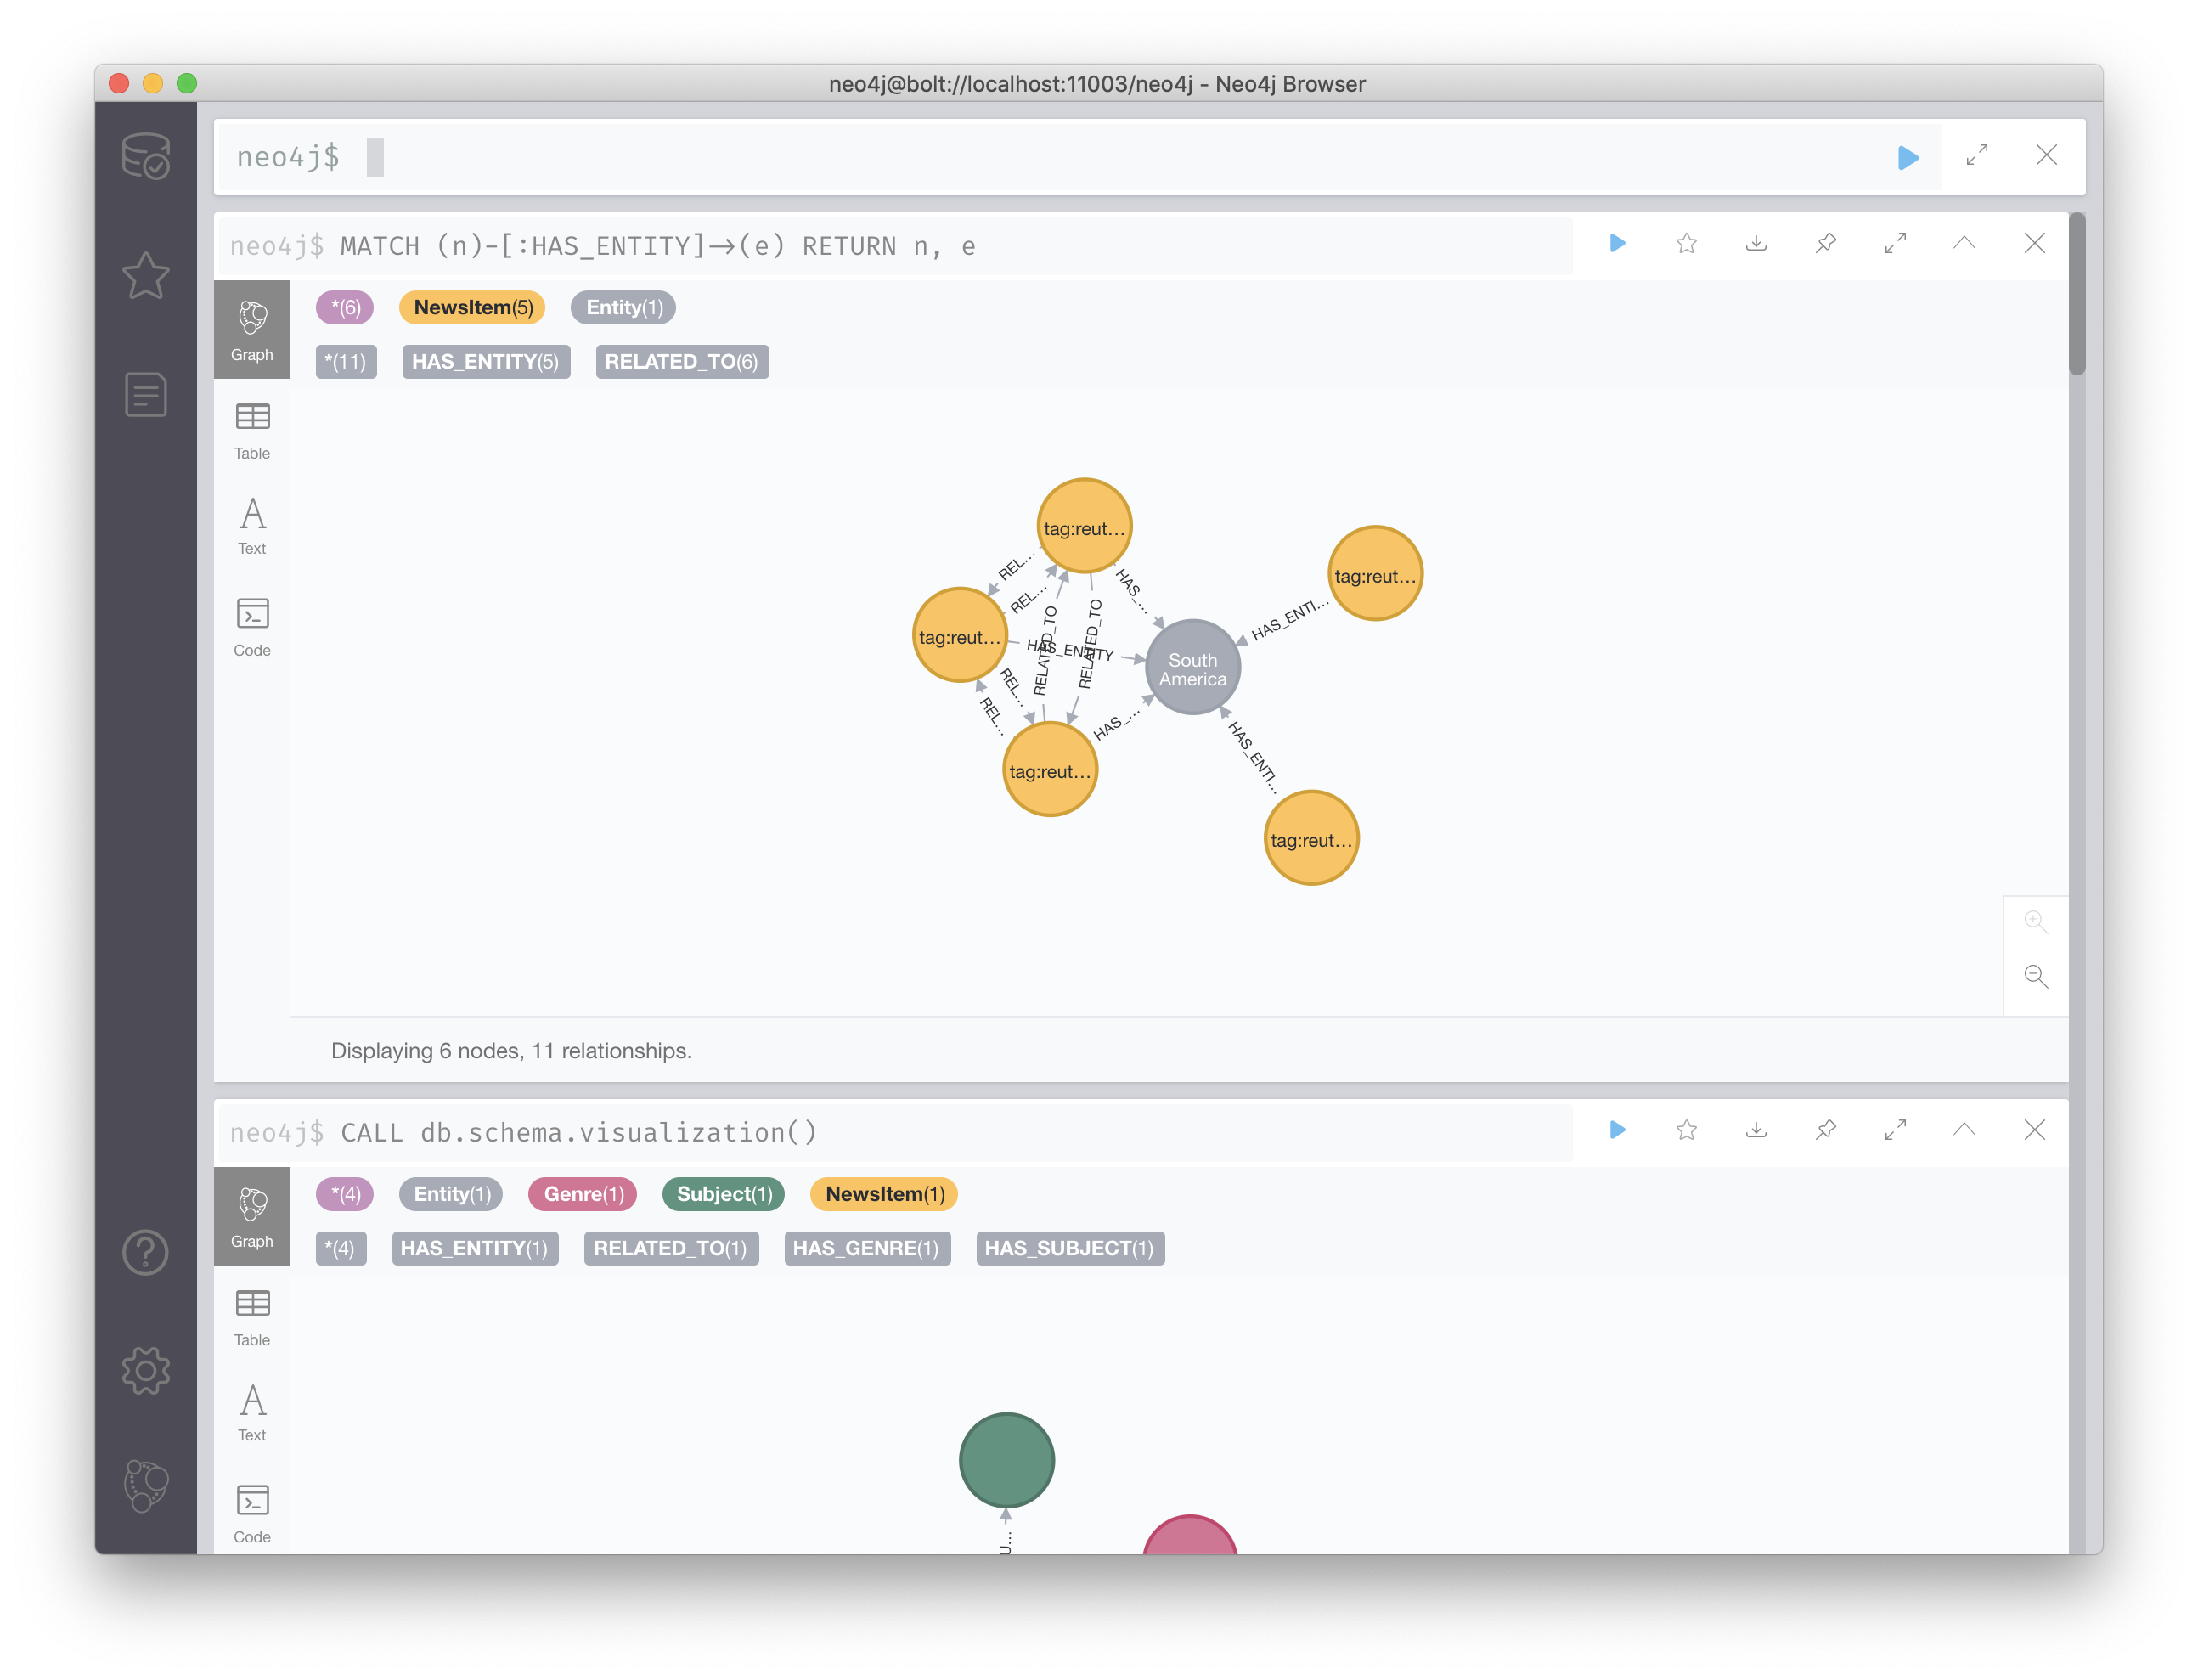
\includegraphics[scale=0.225]{neo4j-cypher-interface}}
\caption{\textit{Cypher query interface of Neo4j Desktop}}
\end{figure}

The end result is an interface by which we can query, for example, all news items that contain a certain entity:

\begin{verbatim}
MATCH (n:NewsItem)-[r:HAS_ENTITY]->(e:Entity {name:"South America"})
RETURN n, r, e
\end{verbatim}

Or all items that are related to each other:

\begin{verbatim}
MATCH (n1:NewsItem)-[r:RELATED_TO]->(n2:NewsItem)
RETURN n1, r, n2
\end{verbatim}




\subsection{Project Plan}
\label{sec:ProjectPlan}
As mentioned in \textit{Figure 1} and the \hyperref[sec:AimsObjectives]{``Aims and Objectives"} section above, an initial investigation and proof of concept is already underway. The first few steps of the project plan aim to consolidate this proof of concept into a verifiable specification, then evaluate semantic technologies and NLP techniques.

The project plan is broken into distinct sequential steps:
\begin{enumerate}
\item{Data exploration} \label{sec:PropDataExploration}
  \begin{enumerate}
  \item Clean and analyse dataset of 59,542 Reuters news items\footnote{Sourced from AWS:\\ \url{https://aws.amazon.com/marketplace/pp/Reuters-News-Archive-30-Days/prodview-qwmkdffmmjesa}}
  \item Review structure of news items, including review of NewsML format and parsing of XML and text
  \end{enumerate}
\item{Literature Review} \label{sec:PropLiteratureReview}
  \begin{enumerate}
  \item Detailed review of knowledge graph, recommendation and NLP literature (\hyperref[sec:LiteratureReview]{See "Literature Review" above})
  \item Identify architecture, techniques, and analyses from literature to be reused in project knowledge graph and experiments
  \end{enumerate}
\item{Data preprocessing and ingestion} \label{sec:PropDataProcessing}
  \begin{enumerate}
  \item Parse Reuters XML docs to produce dataframe\footnote{Proof of concept completed:\\ \url{https://github.com/heychrisek/msc-data-science-project/blob/main/scripts/item_xml_docs_to_csv.py}}
  \item Ingest subset of Reuters dataset into Neo4j\footnote{Proof of concept in progress:\\ \url{https://github.com/heychrisek/msc-data-science-project/blob/main/scripts/csvs_to_neo4j.cypher}}\footnote{https://neo4j.com/labs/apoc/4.1/import/xml/}
  \end{enumerate}
\item{Graph modeling and ST experiments} \label{sec:PropGraphModeling}
  \begin{enumerate}
  \item Build Neo4j/Cypher queries for similar content (e.g., item that’s no more than X steps away via topic or items within date range)
  \item Use Neo4j, APOC, and neosemantics to link Wikidata\footnote{\url{https://neo4j.com/developer/graph-data-science/build-knowledge-graph-nlp-ontologies/}}\footnote{Wikidata script in progress:\\ \url{https://github.com/heychrisek/msc-data-science-project/blob/main/scripts/wikidata_to_wikipedia_url.py}}
  \item Use Neo4j, APOC, and neosemantics to integrate ontology\footnote{\url{https://neo4j.com/developer/graph-data-science/build-knowledge-graph-nlp-ontologies/} and attempt ST experiments to build ontology and link data}
  \item Define graph model\footnote{https://neo4j.com/developer/guide-data-modeling/}. Proof of concept graph model in \textit{Figure 5}.
  \item Complete Knowledge Graph prototype
  \end{enumerate}

\begin{figure}
\centerline{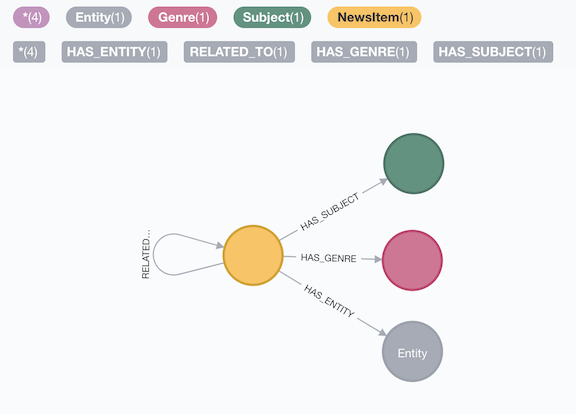
\includegraphics{graph-model}}
\caption{\textit{Proof of concept graph model}}
\end{figure}

\item{Enhance knowledge graph with NLP experiments} \label{sec:PropNLP}
  \begin{enumerate}
  \item NLP models for similarity\footnote{TF-IDF: \url{https://towardsdatascience.com/the-best-document-similarity-algorithm-in-2020-a-beginners-guide-a01b9ef8cf05}}, clustering, keywords, and topics
  \item Language models to predict what a story is about
  \footnote{Resources: \url{http://www.mmds.org} (chapter 3) \\ \url{https://www.youtube.com/watch?v=c6xK9WgRFhI}}
  \item Evaluate NLP experiment
  \item Generate Neo4j knowledge graph relationships between similar items
  \end{enumerate}
\item{[OPTIONAL] Additional considerations if time allows} \label{sec:PropOptional}
  \begin{enumerate}
  \item ML experimentation: probabilistic links and statistical relational learning\cite{nickel2015review}
  \item Prepare a production-ready Neo4j demo, including cloud hosting
  \footnote{\url{https://neo4j.com/developer/guide-cloud-deployment/} \\ \url{https://aws.amazon.com/marketplace/pp/B071P26C9D} \\ \url{https://neo4j.com/developer/neo4j-cloud-aws-ec2-ami/} }
  \item Expose public Cypher query interface/API
  \item Expose web user interface
  \item Build chatbot interface
  \end{enumerate}
\item Finalise written report \label{sec:PropWrittenReport}
  \begin{enumerate}
  \item Evaluate knowledge graph recommendations
  \item Evaluate results of NLP experiments
  \item Evaluate final architecture relative to diagrams below
  \end{enumerate}
\end{enumerate}


\subsection{Risks and Mitigation}
\label{sec:RisksMitigation}

The author anticipates the following risks, with potential impact and mitigation documented if they become a concern.

\begin{enumerate}
\item Risk: Unrealistic scope \\
Impact: Failure to deliver all aspects of project plan \\
Mitigation: Reduce scope to minimum viable project of knowledge graph with some NLP enhancement
\item Risk: Personal circumstances around child's birth in May \\
Impact: May not be possible to strictly follow project timeline \\
Mitigation: The project will follow a Kanban methodology (release as tasks are complete), not waterfall (planned progress in strict sequence)
\item Risk: Limited success of NLP techniques \\
Impact: Failure to generate meaningful recommendations; failure to improve precision/recall \\
Mitigation: We can still learn from experimentation, even if we simply learn what doesn’t work
\item Risk: Insufficient time for step \#6 \\
Impact: Failure to provide enhanced demo or usability \\
Mitigation: Base case is to provide a demo from the local Neo4j Desktop and Cypher query interface
\end{enumerate}


\subsection{Project Timeline}
The following timeline breaks down the approximate intended deliverable by each week. As mentioned in the \hyperref[sec:RisksMitigation]{Risks section}, the intention is not to follow this strictly, but to aim for these delivery dates and adapt as needed.

\begin{itemize}
\item [\textbf{Week}] \textbf{Deliverable}
\item [April 11] Project proposal submission
\item [April 18] Complete initial data exploration/analysis (\hyperref[sec:PropDataExploration]{Project Plan \#1})
\item [April 25] Complete literature review (\hyperref[sec:PropLiteratureReview]{\#2})

\item [May 2]
\item [May 9] Complete initial preprocessing and Neo4j ingestion
\item [May 16] Provide sample Cypher queries
\item [May 23] Complete data processing and ingest (\hyperref[sec:PropDataProcessing]{\#3})
\item [May 30]

\item [June 6]
\item [June 13] Begin graph modeling (\hyperref[sec:PropGraphModeling]{\#4})
\item [June 20]
\item [June 27] Complete knowledge graph prototype (\hyperref[sec:PropGraphModeling]{\#4})

\item [July 4] Begin NLP experiment (\hyperref[sec:PropNLP]{\#5})
\item [July 11]
\item [July 18]
\item [July 25] Complete NLP experiments (\hyperref[sec:PropNLP]{\#5})

\item [August 1] Evaluation of NLP experiments, information retrieval, and recommendations
\item [August 8]
\item [August 15]
\item [August 22]
\item [August 29] Report writing (\hyperref[sec:PropWrittenReport]{\#7})

\item [September 5]
\item [September 12]
\item [September 16] Project submission
\end{itemize}

\subsection{Verification Plan}
The key research question is \textbf{can we build a NewsML to Knowledge Graph pipeline, resulting in a knowledge graph that improves news item recommendations and information retrieval?} Therefore the desired outcome is an affirmative answer to this question, as demonstrated by successful Cypher queries of the Neo4j knowledge graph. This will achieve the aims and objectives of the project

A working graph database will be evidence of successful data cleaning, data ingestion, and data enrichment via NLP techniques. A Cypher script file will be provided to show example queries and results. The enhanced knowledge graph will be made available to demo sample queries, recommendations, and information retrieval.

The completed project will also be verified with a specification, a summary of the NLP techniques applied to the knowledge graph, and an evaluation of how they have performed.

\newpage
\section{Conclusion}

As a MSc Data Science student and a member of the product engineering team at Reuters, the author hopes to (1) understand the news industry, data, and knowledge representation efforts at a deeper level; (2) apply data science techniques to generate insights about the news domain; and (3) as a best case scenario, create meaningful value for Reuters and the broader media.

This project is the culmination of the MSc Data Science degree and therefore aims to combine key learnings from data science, semantic technology, natural language processing, and information retrieval into a single research and software development project. Completing this project and achieving the \hyperref[sec:AimsObjectives]{aims and objectives} will provide experience and build confidence with technologies including Neo4j, Cypher, Python, OWL, and RDF.

\newpage
\section{Glossary}
\begin{itemize}
\item KG - Knowledge graph
\item ML - Machine learning
\item NewsML\footnote{\url{https://iptc.org/standards/newsml-g2/}} - XML format for news items and metadata
\item OWL - Web Ontology Language
\item NER - Named entity recognition
\item NLP - Natural language processing
\item SRL - Statistical relational learning
\item ST - Semantic technology
\item XML - Extensible Markup Language format for encoding documents
\end{itemize}

\newpage
\bibliographystyle{abbrv}
\bibliography{proposal}

\end{document}  